
\documentclass[paper=letter,11pt]{scrartcl}

\KOMAoptions{headinclude=true, footinclude=false}
\KOMAoptions{DIV=14, BCOR=5mm}
\KOMAoptions{numbers=noendperiod}
\KOMAoptions{parskip=half}
\addtokomafont{disposition}{\rmfamily}
\addtokomafont{part}{\LARGE}
\addtokomafont{descriptionlabel}{\rmfamily}
%\setkomafont{pageheadfoot}{\normalsize\sffamily}
\setkomafont{pagehead}{\normalsize\rmfamily}
%\setkomafont{publishers}{\normalsize\rmfamily}
\setkomafont{caption}{\normalfont\small}
\setcapindent{0pt}
\deffootnote[1em]{1em}{1em}{\textsuperscript{\thefootnotemark}\ }


\usepackage{amsmath}
\usepackage[varg]{txfonts}
\usepackage[T1]{fontenc}
\usepackage{graphicx}
\usepackage{xcolor}
\usepackage[american]{babel}
% hyperref is needed in many places, so include it here
\usepackage{hyperref}

\usepackage{xspace}
\usepackage{multirow}
\usepackage{float}


\usepackage{braket}
\usepackage{bbm}
\usepackage{relsize}
\usepackage{tcolorbox}

\def\ketY{\ensuremath{\ket {\Psi}}}
\def\iGeV{\ensuremath{\textrm{GeV}^{-1}}}
%\def\mp{\ensuremath{m_{\textrm{proton}}}}
\def\rp{\ensuremath{r_{\textrm{proton}}}}
\def\me{\ensuremath{m_{\textrm{electron}}}}
\def\aG{\ensuremath{\alpha_G}}
\def\rAtom{\ensuremath{r_{\textrm{atom}}}}
\def\rNucl{\ensuremath{r_{\textrm{nucleus}}}}
\def\GN{\ensuremath{\textrm{G}_\textrm{N}}}
\def\ketX{\ensuremath{\ket{\vec{x}}}}
\def\ve{\ensuremath{\vec{\epsilon}}}


\def\ABCDMatrix{\ensuremath{\begin{pmatrix} A &  B  \\ C  & D \end{pmatrix}}}
\def\xyprime{\ensuremath{\begin{pmatrix} x' \\ y' \end{pmatrix}}}
\def\xyprimeT{\ensuremath{\begin{pmatrix} x' &  y' \end{pmatrix}}}
\def\xy{\ensuremath{\begin{pmatrix} x \\ y \end{pmatrix}}}
\def\xyT{\ensuremath{\begin{pmatrix} x & y \end{pmatrix}}}

\def\IMatrix{\ensuremath{\begin{pmatrix} 0 &  1  \\ -1  & 0 \end{pmatrix}}}
\def\IBoostMatrix{\ensuremath{\begin{pmatrix} 0 &  1  \\ 1  & 0 \end{pmatrix}}}
\def\JThree{\ensuremath{\begin{pmatrix}    0 & -i & 0  \\ i & 0  & 0 \\ 0 & 0 & 0 \end{pmatrix}}} 
\def\JTwo{\ensuremath{\begin{bmatrix}    0 & 0 & -i  \\ 0 & 0  & 0 \\ i & 0 & 0 \end{bmatrix}}}
\def\JOne{\ensuremath{\begin{bmatrix}    0 & 0 & 0  \\ 0 & 0  & -i \\ 0 & i & 0 \end{bmatrix}}}
\def\etamn{\ensuremath{\eta_{\mu\nu}}}
\def\Lmn{\ensuremath{\Lambda^\mu_\nu}}
\def\dmn{\ensuremath{\delta^\mu_\nu}}
\def\wmn{\ensuremath{\omega^\mu_\nu}}
\def\be{\begin{equation*}}
\def\ee{\end{equation*}}
\def\bea{\begin{eqnarray*}}
\def\eea{\end{eqnarray*}}
\def\bi{\begin{itemize}}
\def\ei{\end{itemize}}
\def\fmn{\ensuremath{F_{\mu\nu}}}
\def\fMN{\ensuremath{F^{\mu\nu}}}
\def\bc{\begin{center}}
\def\ec{\end{center}}
\def\nus{$\nu$s}

\def\adagger{\ensuremath{a_{p\sigma}^\dagger}}
\def\lineacross{\noindent\rule{\textwidth}{1pt}}

\newcommand{\multiline}[1] {
\begin{tabular} {|l}
#1
\end{tabular}
}

\newcommand{\multilineNoLine}[1] {
\begin{tabular} {l}
#1
\end{tabular}
}



\newcommand{\lineTwo}[2] {
\begin{tabular} {|l}
#1 \\
#2
\end{tabular}
}

\newcommand{\rmt}[1] {
\textrm{#1}
}


%
% Units
%
\def\m{\ensuremath{\rmt{m}}}
\def\GeV{\ensuremath{\rmt{GeV}}}
\def\pt{\ensuremath{p_\rmt{T}}}


\def\parity{\ensuremath{\mathcal{P}}}

\usepackage{cancel}
\usepackage{ mathrsfs }
\def\bigL{\ensuremath{\mathscr{L}}}

\usepackage{ dsfont }



\usepackage{fancyhdr}
\fancyhf{}

\usepackage{braket}

\def\ketY{\ensuremath{\ket {\Psi}}}
\def\iGeV{\ensuremath{\textrm{GeV}^{-1}}}
\def\mp{\ensuremath{m_{\textrm{proton}}}}
\def\rp{\ensuremath{r_{\textrm{proton}}}}
\def\me{\ensuremath{m_{\textrm{electron}}}}
\def\aG{\ensuremath{\alpha_G}}
\def\rAtom{\ensuremath{r_{\textrm{atom}}}}
\def\rNucl{\ensuremath{r_{\textrm{nucleus}}}}
\def\GN{\ensuremath{\textrm{G}_\textrm{N}}}

\def\be{\begin{equation*}}
\def\ee{\end{equation*}}


\usepackage{fancyhdr}
\usepackage{cancel}
\usepackage{ mathrsfs }





\fancyhf{}
\lhead{\Large 33-444} % \hfill Introduction to Particle Physics \hfill Spring 2019}
\chead{\Large Introduction to Particle Physics} % \hfill Spring 2019}
\rhead{\Large Spring 2019} % \hfill Introduction to Particle Physics \hfill Spring 2019}
\begin{document}
\thispagestyle{fancy}





%\begin{tabular}{c}
%{\large 33-444 \hfill Intro To Particle \hfill Spring 2019\\}
%\hline 
%\end{tabular}

\begin{center}
{\huge \textbf{Midterm}}
\large

\end{center}

{\large


\textbf{1) Why are energy and momentum conserved in the Standard Model ?  What would it mean if we found evidence for non-conservation of Energy ? What about non-conservation of Momentum? }\hfill \textit{(3 points)}\\

\vspace{3in}

\textbf{2) What are three major consequences of combining QM and Relativity?}\hfill \textit{(3 points)}\\

\vspace{3in}

\clearpage
\textbf{3)  GZK cutoff energy} \hfill \textit{(5 points)}\\
High-energy cosmic rays (high energy protons), lose energy by interacting with CMB photons by producing a neutral pion:
\be
p+\gamma_{\mathrm{CMB}} \rightarrow p+\pi_0.
\ee
The proton energy at which this process can occur is called the GZK cutoff. 
Estimate the GZK cutoff energy.
The energy of CMB photons is $10^{-13}$ GeV (which follows from the measurement of CMB temperature of about 2.7 K).
Use 0.1 GeV for the mass of the pion and 1 GeV for the mass of the proton

\vspace{4in}


\textbf{4) Neutrino masses. The seesaw mechanism is a proposed source for neutrino masses. In this scenario the neutrino would get a mass from the following diagram.} \hfill \textit{(2 points)}\\
Describing the interaction of a neutrino($\nu$) with a Higgs boson ($h$).
What is the dimension of the coupling constant associated with this diagram ?

\begin{figure}[h!]
\centering
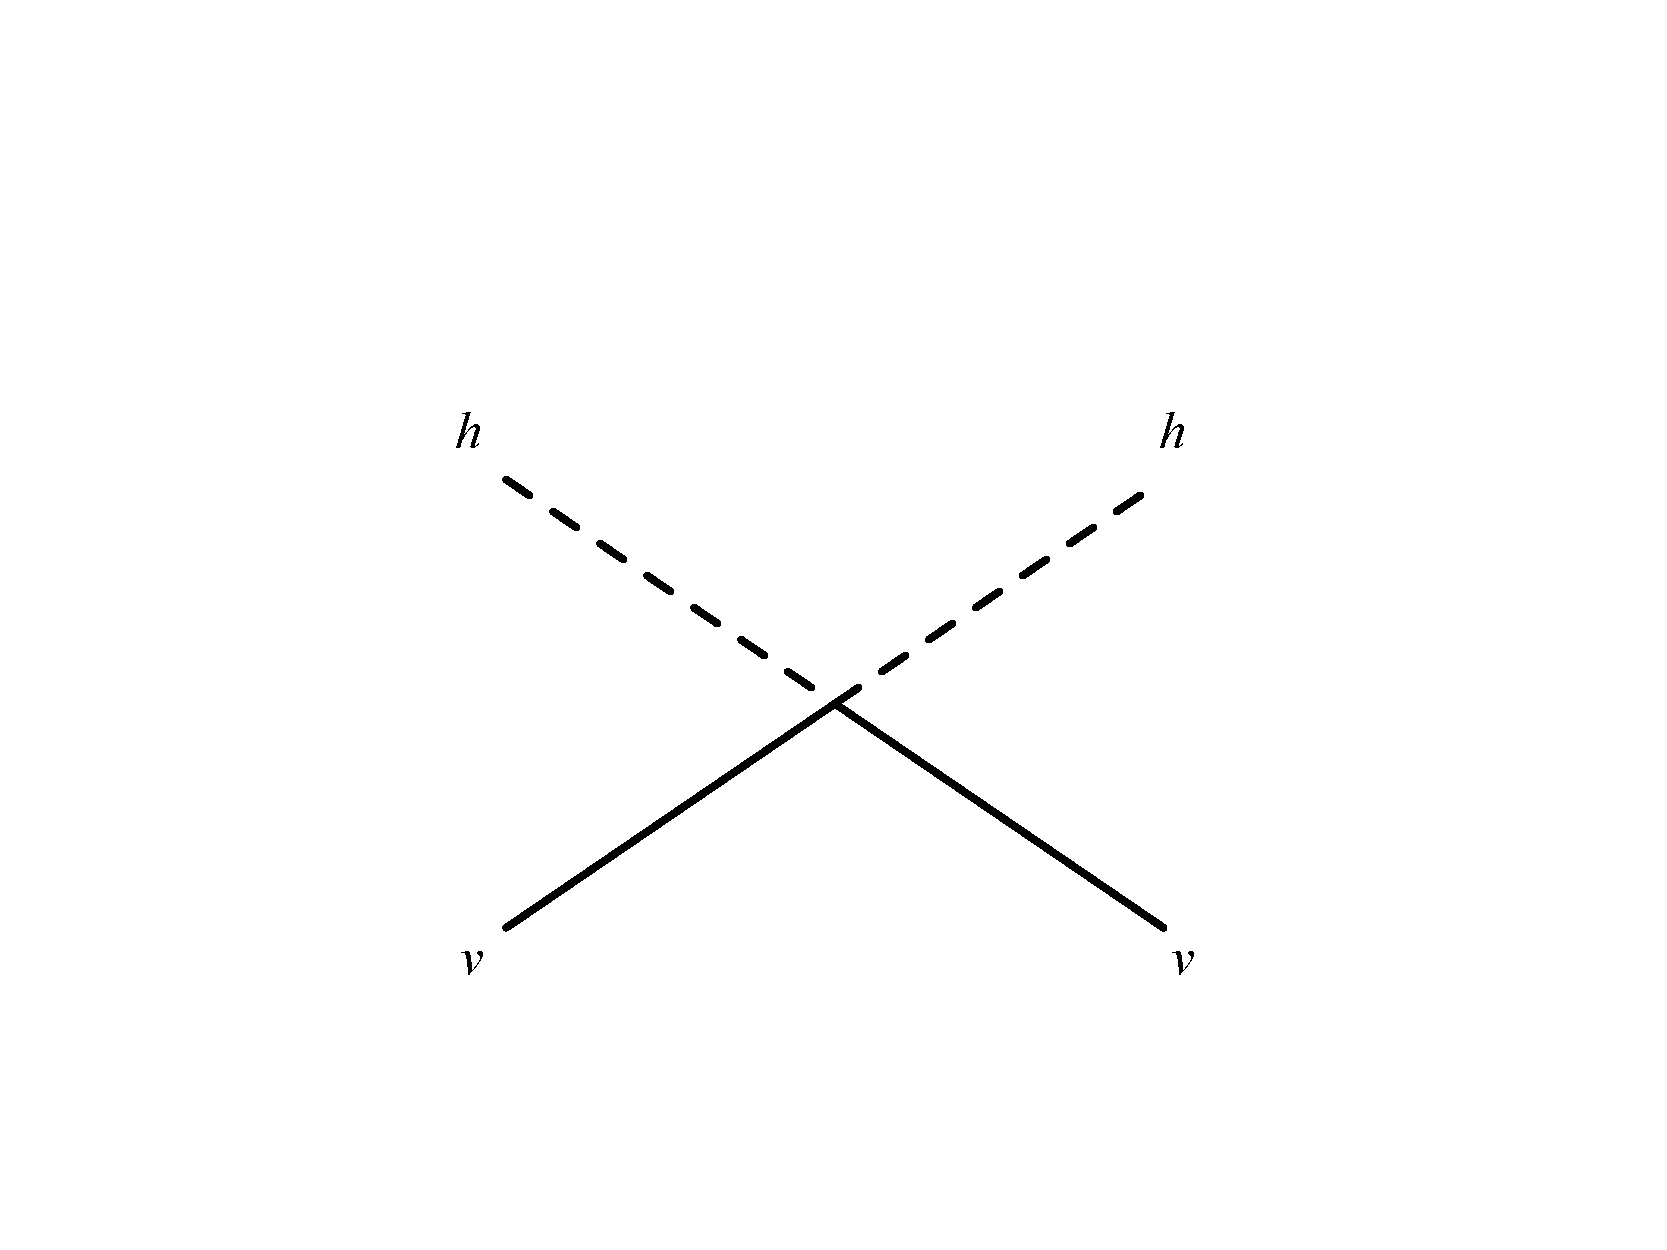
\includegraphics[width=0.3\textwidth]{./NuMassDiagram.pdf}
\end{figure}


\clearpage


\textbf{5) Why do we label particle states by momentum? } \hfill \textit{(2 points)}\\

\vspace{2in}


\textbf{6) Why is the weak interaction so much weaker than the electromagnetic interaction at low energies?}\hfill \textit{(2 points)}\\

\vspace{2in}


\textbf{7) What are three restrictions to particle interactions that are a consequence gauge invariance ? }\hfill \textit{(3 points)}\\


\vspace{2in}

\clearpage

\textbf{8) Lorentz Transforms } \hfill \textit{(5 points)}\\
\begin{itemize}
\item[a)] How does a massive particle $\ket{p^\mu,\sigma}$ transform under a general Lorentz transformation ($\Lambda_\mu^\nu$)  ?
\vspace*{1in}
\item[b)] How does a massive particle $\ket{p^\mu,\sigma}$ transform under a little group transformation ($W_\mu^\nu$)  ?
\vspace*{1in}
\item[c)] How does a mass-less particle $\ket{p^\mu,\sigma}$ transform under a general Lorentz transformation ($\Lambda_\mu^\nu$)  ?
\vspace*{1in}
\item[d)] How does a mass-less particle $\ket{p^\mu,\sigma}$ transform under a little group transformation ($W_\mu^\nu$)  ?
\vspace*{1in}
\end{itemize}




\clearpage

\textbf{9) $ee\rightarrow\tau\tau$ scattering } \hfill \textit{(5 points)}\\
\begin{itemize}
\item[a)]{
At high energy ($E_{CM} >> m_\tau$), what is the dependence of the $ee\rightarrow\tau\tau$ cross section on $E_{CM}$ ?
\vspace*{1in}
}

%\item[b)]{
%At high energy ($E_{CM} >> m_\tau$), derive the dependence of the cross section on scattering angle $\theta$.
%\vspace*{4in}
%}

\item[b)]{
Sketch a graph of $\frac{\sigma(ee\rightarrow\tau\tau)}{\sigma(ee\rightarrow\mu\mu)}$ as a function of $E_{CM}$ from $2\times m_{\mu}$ to 1 TeV (= 1000 GeV).
\vspace*{1in}
}
\end{itemize}

%scalar QED. treat electron as scalar, photon as massless spin 1 particle
%  ee->ee scattering: Draw diagrmas, what are the associated matrix elements.


%what about ee->tau tau? again at high energy where $E_{CM}$ >> tau tau.

% work out the differential cross section ee->tautau in the massless limit.

\clearpage

\textbf{10) Muon decays: } \hfill \textit{(10 points)}\\
\begin{itemize}
  \item[a)]{ The muon decays via the weak interaction,  At low energy ($E << m_W$), this can be approximated as a point-like interaction. 
  Draw the diagram describing muon decay to an electron assuming a point-like weak interaction.
\vspace*{1.5in}
}
  \item[b)]{ What are the dimensions of the coupling constant, associated to this diagram  ?
\vspace*{1.0in}
  }
  \item[c)] How does the decay rate $\Gamma$ (decays/unit time)  depend on the muon mass ? 
\vspace*{1.0in}
  \item[d)]{ The muon has a mass of $\sim$0.1 GeV and a lifetime of $\sim 1 \mu s$. The tau lepton has a mass of {$\sim$1 GeV}. Estimate the lifetime of the tau lepton in $\mu s$.
\vspace*{2.4in}
}
  \item[e)] {Suppose that the photon could couple at the same vertex to the muon and the electron. Then the muon could decay as $\mu\rightarrow e \gamma$. 
  Estimate the ratio of the $\mu$ lifetime in this world to that in our world without this interaction.
  \vspace*{3.0in}
  }
\end{itemize}

\textbf{11) Can the SM have interactions between fermions and massive particles with Spin 3 ? If not, why not.  What about interactions between mass-less Spin 3 particles and fermions ? If not, why not. }\hfill \textit{(2 points)}\\

\vspace*{1.5in}

\textbf{12) Yukawa’s Theory.}\hfill \textit{(2 points)}
In the 1930s, Hideki Yukawa predicted the existence of a new particle, now called the pion, which is responsible for binding protons and neutrons together in atomic nuclei. 
Estimate the mass of the pion from the assumed range of the force. ($10^{-15}$ meters). 
Express the mass in GeV.

\clearpage



\textbf{13) List or draw a diagram of the particles in the Standard model. } \hfill \textit{(3 points)}\\
What is the spin of each particle ?

\vspace*{3in}

\textbf{14)  How many generators does the Lorentz group have ? }\hfill \textit{(2 points)}\\
What transformations do they correspond to ?

\vspace*{2in}

\textbf{15) Neutrino interactions } \hfill \textit{(2 points)}\\
Assuming lepton universality, would you expect a difference between the way $\nu_e$ and $\nu_\mu$ interact with matter ?
Justify your answer by drawing the leading order diagrams for $\nu_e + e \rightarrow \nu_e + e$  and $\nu_\mu + e \rightarrow \nu_\mu + e$.

\vspace*{0.25in}


\clearpage

\textbf{16) A new force. } \hfill \textit{(5 points)}\\
Assume there is another force of nature felt by electrons associated with the exchange of a new X boson of mass 1 TeV (= 1000 GeV).
\begin{itemize}
\item[a)]{ Estimate an upper limit on the range of this new force in meters.
\vspace{2in}
}
%\item[b)]{ Assume muons also interact with this new boson. How could you determine the spin of X ?}
\item[b)]{ Assume that this new X boson could also decay to spin-1/2 dark matter particles $\psi_{DM}$. At low energies (<< 1 TeV) the X interaction can be described by a point-like interaction. Estimate the coupling constant associated to dark matter scattering $e \psi_{DM} \rightarrow e \psi_{DM}$.   (Assume the X coupling at high energies is the same as for EM)  }
\vspace*{2in}
\item[c)]{ Assume there was a direct $X\rightarrow e\mu$ interaction. This would allow the muon to decay via $\mu^- \rightarrow e^-e^+e^-$. Draw the corresponding diagram and estimate the impact of the muon lifetime from this process.  How does it compare to the lifetime in the standard model?     }
\end{itemize}






} % Begning Large
\end{document}
